\section{ERROR ALLOCATION AND SELECTED LABEL ACQUISITION}
\label{app:allocation}
\paragraph{Stratum-size allocation.}
In Lemma~\ref{lem:stratified}, the realized $m_h$ need not be fixed before normal roles are drawn. They are fixed after conditioning on the stratum role counts $\mathcal K$. Setting $\alpha_h=\alpha m_h/m$ therefore gives
\[
\E[\FDP_{\rm union}\mid\mathcal F,\mathcal K]
\le \sum_{h:m_h>0}\frac{\alpha m_h}{m}\frac{m_{0h}}{m_h}
=\alpha\frac{m_0}{m}.
\]
This is an allocation rule, not a power ordering relative to equal allocation.

\paragraph{One BH across stratified ranks.}
Suppose normal reference revelation has a fixed probability $\rho_h$ within each fixed stratum, independently across nodes. For a feasible assignment of normal identities to test, reference and unused roles, its probability conditional on $\mathcal F$ is
\[
\binom Nt^{-1}\prod_h\rho_h^{n_h}(1-\rho_h)^{u_h}.
\]
Given $\mathcal K$, this is constant over a Cartesian product of the feasible within-stratum assignments. Its normalizing constant factors over that product. Consequently the within-stratum role assignments are independent under this conditioning. This independence follows from randomized roles on the fixed graph, not from independence of graph observations. It would not hold automatically for an arbitrary adaptive acquisition policy.

In each stratum, introduce independent random orderings of calibration and null-test positions as in the proof of Lemma~\ref{lem:stratified}. The conditional exchangeability theorem supplies super-uniform null ranks and PRDS within each block~\citep[Theorem 3.3]{marandon2024adaptive}. An empty-reference block has constant p-values equal to one. Independent PRDS blocks are jointly PRDS: for a null coordinate in block $h$ and any coordinatewise increasing set $A$, fix the other blocks. Its section in block $h$ is increasing, so its conditional probability is nondecreasing in that null p-value. Average over the independent other blocks; their law does not change with the conditioned coordinate. This preserves the monotonicity. Thus one BH at $\alpha$ on all stratum-wise p-values satisfies
\[
\E[\FDP_{\rm pooled\ strata}\mid\mathcal F,\mathcal K]
\le\alpha m_0/m.
\]
The artificial ordering of positions changes neither the rejection set nor FDP. Averaging over counts preserves the bound. This result strengthens the allocation argument only for the specified product sampling design; the earlier sum-FDP argument remains applicable without cross-stratum independence.

\paragraph{Known-propensity weighting.}
For the biased-acquisition experiment, strata and probabilities are fixed using only training labels and graph features. Assign a prescribed total number of normal test positions uniformly, then acquire each remaining normal with probability $\rho(v)=\rho_{h(v)}>0$. Consider one designated null test position. Condition on all other null test identities, the unordered union $S$ of its node and calibration nodes, and the unused nodes; do not additionally fix this designated position's stratum. For a possible target $j\in S$, assignment probability is proportional to
\[
\prod_{i\in S\setminus\{j\}}\rho(i)
=\frac{\prod_{i\in S}\rho(i)}{\rho(j)}.
\]
Uniform test-position assignment and the probabilities of unused nodes contribute common factors. Conditional target mass is therefore proportional to $w(j)=1/\rho(j)$. Summing this mass over nodes with score at least the target score yields
\[
p_w(v)=\frac{w(v)+\sum_{u\in C}w(u)\ind\{s(u)\ge s(v)\}}
{w(v)+\sum_{u\in C}w(u)}.
\]
The cumulative-mass argument gives marginal null super-uniformity; an empty reference returns one. This is the weighted-exchangeability principle~\citep{tibshirani2019conformal} applied to the acquisition design. BY at $\alpha/\sum_{j=1}^m1/j$ consequently controls FDR under arbitrary p-value dependence~\citep{benjamini2001control}. Weighted BH is retained as a descriptive comparator: the marginal argument does not establish its joint PRDS condition. These probabilities are known by design, not estimated propensities for an arbitrary analyst policy.

\begin{figure*}[t]
\centering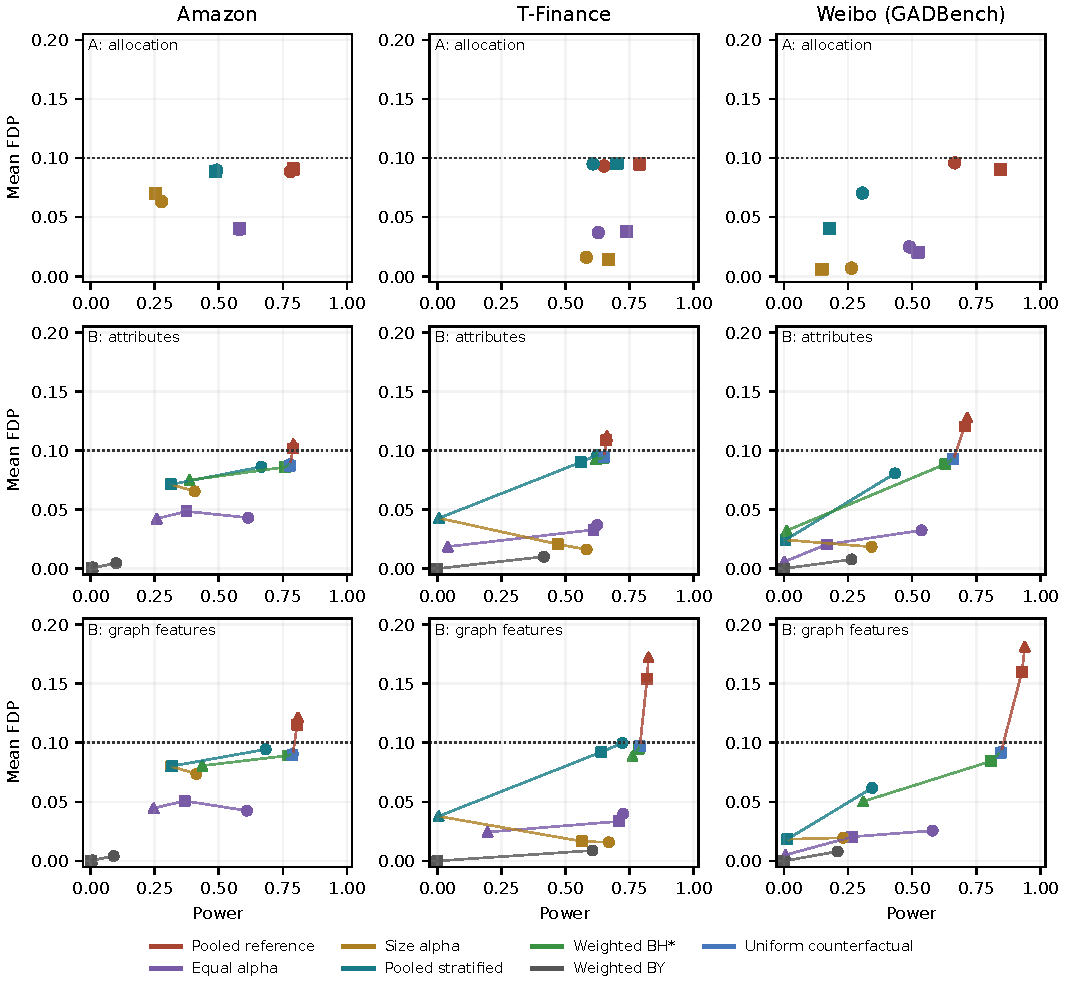
\includegraphics[width=\textwidth]{allocation_acquisition.pdf}
\caption{FDP versus power for the prespecified 80/20 partition. Top: uniform acquisition at half revelation, comparing allocation rules; circles/squares denote attribute/graph scorers. Middle and bottom: biased acquisition with attribute and graph scorers. Circles, squares and triangles follow neutral, moderate and severe acquisition bias; lines connect those settings, not a tuned frontier. Dotted lines mark nominal $0.10$. Weighted BH* has no joint guarantee established here. Uniform acquisition is a counterfactual, not an available reference within the biased-design scenario. All methods share scores and test identities; means include abstentions.}
\label{fig:allocationfull}
\end{figure*}

The follow-up protocol was frozen after the equal-alpha results, before these variants were evaluated. It is an exploratory follow-up. Phase A reproduces 5,400 previously stored outcomes before comparing allocations. Phase B fixes exposure using only training labels and graph degree, then independently acquires each non-test node's label with the stated stratum probability. Acquired anomalies count toward label cost but are not normal references. Strata are never updated with newly acquired labels. The uniform counterfactual uses the deployment-universe mean acquisition probability, fixed before normal-role assignment; costs are close in expectation, not matched exactly per realization. Each phase retains all ten training seeds and five splits; phase B adds ten acquisition repetitions. The full ledger has 135,000 procedure evaluations.

All means include abstentions. Pointwise paired intervals over ten seed averages are supplied in the result CSVs; they do not quantify cross-graph uncertainty. Exact small-design checks include 6,246 conditional block assignments with nonzero false-discovery events, and 11,264 unequal-propensity assignments for marginal weighted ranks. These checks support implementation verification and do not replace the argument above.

\begin{table*}[t]\centering\scriptsize\setlength{\tabcolsep}{3pt}
\caption{Amazon, allocation: mean FDP / power. Every declared partition and setting is shown. For acquisition, neu/mod/sev denote $(\rho_L,\rho_H)=(.5,.5),(.5,.1),(.5,.025)$. W-BH* is descriptive; its marginal-rank argument is not a BH guarantee. Uniform is a counterfactual acquisition design.}
\begin{tabular}{lllrrrrr}\toprule Score & Strata & Setting & Pooled & Equal & Size & Joint & Low only\\\midrule
Attr. & Zero & 0.25 & $0.091/0.779$ & $0.039/0.567$ & $0.072/0.655$ & $0.081/0.755$ & $0.093/0.679$ \\
Attr. & Zero & 0.50 & $0.089/0.779$ & $0.042/0.651$ & $0.078/0.714$ & $0.088/0.774$ & $0.140/0.770$ \\
Attr. & Zero & 1.00 & $0.092/0.783$ & $0.044/0.694$ & $0.088/0.758$ & $0.092/0.781$ & $0.198/0.807$ \\
Attr. & 80/20 & 0.25 & $0.091/0.779$ & $0.036/0.530$ & $0.055/0.182$ & $0.070/0.404$ & $0.110/0.793$ \\
Attr. & 80/20 & 0.50 & $0.089/0.779$ & $0.039/0.581$ & $0.063/0.277$ & $0.090/0.492$ & $0.114/0.797$ \\
Attr. & 80/20 & 1.00 & $0.092/0.783$ & $0.038/0.637$ & $0.054/0.287$ & $0.094/0.551$ & $0.118/0.800$ \\
Graph & Zero & 0.25 & $0.089/0.778$ & $0.047/0.572$ & $0.073/0.645$ & $0.081/0.751$ & $0.085/0.675$ \\
Graph & Zero & 0.50 & $0.091/0.791$ & $0.045/0.665$ & $0.080/0.716$ & $0.089/0.781$ & $0.118/0.756$ \\
Graph & Zero & 1.00 & $0.091/0.793$ & $0.046/0.697$ & $0.088/0.764$ & $0.089/0.789$ & $0.155/0.791$ \\
Graph & 80/20 & 0.25 & $0.089/0.778$ & $0.038/0.509$ & $0.065/0.212$ & $0.082/0.457$ & $0.127/0.813$ \\
Graph & 80/20 & 0.50 & $0.091/0.791$ & $0.040/0.579$ & $0.070/0.252$ & $0.089/0.487$ & $0.132/0.814$ \\
Graph & 80/20 & 1.00 & $0.091/0.793$ & $0.034/0.639$ & $0.073/0.258$ & $0.096/0.516$ & $0.139/0.818$ \\
\bottomrule\end{tabular}\end{table*}

\begin{table*}[t]\centering\scriptsize\setlength{\tabcolsep}{3pt}
\caption{T-Finance, allocation: mean FDP / power. Every declared partition and setting is shown. For acquisition, neu/mod/sev denote $(\rho_L,\rho_H)=(.5,.5),(.5,.1),(.5,.025)$. W-BH* is descriptive; its marginal-rank argument is not a BH guarantee. Uniform is a counterfactual acquisition design.}
\begin{tabular}{lllrrrrr}\toprule Score & Strata & Setting & Pooled & Equal & Size & Joint & Low only\\\midrule
Attr. & Zero & 0.25 & $0.093/0.650$ & $0.046/0.633$ & $0.051/0.638$ & $0.090/0.658$ & $0.067/0.627$ \\
Attr. & Zero & 0.50 & $0.093/0.651$ & $0.045/0.633$ & $0.056/0.646$ & $0.092/0.660$ & $0.067/0.626$ \\
Attr. & Zero & 1.00 & $0.095/0.652$ & $0.045/0.629$ & $0.063/0.647$ & $0.093/0.658$ & $0.071/0.633$ \\
Attr. & 80/20 & 0.25 & $0.093/0.650$ & $0.037/0.623$ & $0.014/0.567$ & $0.093/0.607$ & $0.119/0.665$ \\
Attr. & 80/20 & 0.50 & $0.093/0.651$ & $0.037/0.628$ & $0.016/0.581$ & $0.095/0.608$ & $0.127/0.669$ \\
Attr. & 80/20 & 1.00 & $0.095/0.652$ & $0.037/0.629$ & $0.015/0.577$ & $0.100/0.603$ & $0.138/0.675$ \\
Graph & Zero & 0.25 & $0.092/0.787$ & $0.043/0.744$ & $0.048/0.752$ & $0.092/0.775$ & $0.123/0.803$ \\
Graph & Zero & 0.50 & $0.095/0.789$ & $0.044/0.751$ & $0.056/0.766$ & $0.095/0.784$ & $0.122/0.803$ \\
Graph & Zero & 1.00 & $0.099/0.792$ & $0.046/0.753$ & $0.065/0.776$ & $0.098/0.789$ & $0.121/0.804$ \\
Graph & 80/20 & 0.25 & $0.092/0.787$ & $0.038/0.731$ & $0.012/0.648$ & $0.090/0.690$ & $0.182/0.827$ \\
Graph & 80/20 & 0.50 & $0.095/0.789$ & $0.038/0.737$ & $0.014/0.668$ & $0.095/0.701$ & $0.192/0.830$ \\
Graph & 80/20 & 1.00 & $0.099/0.792$ & $0.038/0.738$ & $0.013/0.676$ & $0.101/0.708$ & $0.202/0.834$ \\
\bottomrule\end{tabular}\end{table*}

\begin{table*}[t]\centering\scriptsize\setlength{\tabcolsep}{3pt}
\caption{Weibo (GADBench), allocation: mean FDP / power. Every declared partition and setting is shown. For acquisition, neu/mod/sev denote $(\rho_L,\rho_H)=(.5,.5),(.5,.1),(.5,.025)$. W-BH* is descriptive; its marginal-rank argument is not a BH guarantee. Uniform is a counterfactual acquisition design.}
\begin{tabular}{lllrrrrr}\toprule Score & Strata & Setting & Pooled & Equal & Size & Joint & Low only\\\midrule
Attr. & Zero & 0.25 & $0.093/0.664$ & $0.025/0.478$ & $0.011/0.260$ & $0.048/0.284$ & $0.164/0.758$ \\
Attr. & Zero & 0.50 & $0.096/0.666$ & $0.036/0.537$ & $0.020/0.443$ & $0.086/0.466$ & $0.181/0.779$ \\
Attr. & Zero & 1.00 & $0.093/0.664$ & $0.042/0.559$ & $0.032/0.519$ & $0.096/0.536$ & $0.198/0.795$ \\
Attr. & 80/20 & 0.25 & $0.093/0.664$ & $0.017/0.401$ & $0.001/0.013$ & $0.010/0.049$ & $0.168/0.764$ \\
Attr. & 80/20 & 0.50 & $0.096/0.666$ & $0.025/0.489$ & $0.007/0.263$ & $0.070/0.306$ & $0.189/0.787$ \\
Attr. & 80/20 & 1.00 & $0.093/0.664$ & $0.026/0.495$ & $0.009/0.377$ & $0.089/0.384$ & $0.216/0.811$ \\
Graph & Zero & 0.25 & $0.094/0.845$ & $0.030/0.571$ & $0.012/0.286$ & $0.056/0.322$ & $0.253/0.966$ \\
Graph & Zero & 0.50 & $0.090/0.846$ & $0.029/0.630$ & $0.016/0.457$ & $0.072/0.474$ & $0.280/0.972$ \\
Graph & Zero & 1.00 & $0.093/0.848$ & $0.035/0.673$ & $0.029/0.622$ & $0.090/0.637$ & $0.311/0.978$ \\
Graph & 80/20 & 0.25 & $0.094/0.845$ & $0.023/0.474$ & $0.005/0.066$ & $0.019/0.093$ & $0.258/0.969$ \\
Graph & 80/20 & 0.50 & $0.090/0.846$ & $0.020/0.523$ & $0.006/0.148$ & $0.041/0.178$ & $0.290/0.974$ \\
Graph & 80/20 & 1.00 & $0.093/0.848$ & $0.023/0.567$ & $0.007/0.204$ & $0.061/0.249$ & $0.317/0.978$ \\
\bottomrule\end{tabular}\end{table*}

\begin{table*}[t]\centering\scriptsize\setlength{\tabcolsep}{3pt}
\caption{Amazon, acquisition: mean FDP / power. Every declared partition and setting is shown. For acquisition, neu/mod/sev denote $(\rho_L,\rho_H)=(.5,.5),(.5,.1),(.5,.025)$. W-BH* is descriptive; its marginal-rank argument is not a BH guarantee. Uniform is a counterfactual acquisition design.}
\begin{tabular}{lllrrrrrrr}\toprule Score & Strata & Setting & Pooled & Equal & Size & Joint & W-BH* & W-BY & Uniform\\\midrule
Attr. & Zero & neu & $0.088/0.779$ & $0.044/0.635$ & $0.050/0.621$ & $0.086/0.775$ & $0.088/0.779$ & $0.005/0.100$ & $0.088/0.779$ \\
Attr. & Zero & mod & $0.085/0.774$ & $0.047/0.455$ & $0.042/0.463$ & $0.079/0.728$ & $0.084/0.753$ & $0.000/0.001$ & $0.086/0.772$ \\
Attr. & Zero & sev & $0.083/0.771$ & $0.038/0.216$ & $0.026/0.172$ & $0.032/0.194$ & $0.067/0.345$ & $0.000/0.002$ & $0.085/0.770$ \\
Attr. & 80/20 & neu & $0.088/0.779$ & $0.043/0.615$ & $0.065/0.406$ & $0.086/0.666$ & $0.088/0.779$ & $0.005/0.100$ & $0.088/0.779$ \\
Attr. & 80/20 & mod & $0.102/0.789$ & $0.048/0.374$ & $0.071/0.311$ & $0.071/0.313$ & $0.086/0.757$ & $0.001/0.004$ & $0.087/0.778$ \\
Attr. & 80/20 & sev & $0.105/0.791$ & $0.042/0.258$ & $0.071/0.311$ & $0.071/0.311$ & $0.075/0.386$ & $0.001/0.008$ & $0.087/0.777$ \\
Graph & Zero & neu & $0.090/0.789$ & $0.045/0.639$ & $0.051/0.617$ & $0.088/0.783$ & $0.090/0.789$ & $0.004/0.090$ & $0.090/0.789$ \\
Graph & Zero & mod & $0.082/0.778$ & $0.048/0.466$ & $0.044/0.469$ & $0.081/0.739$ & $0.087/0.767$ & $0.000/0.001$ & $0.090/0.783$ \\
Graph & Zero & sev & $0.079/0.775$ & $0.038/0.209$ & $0.025/0.153$ & $0.030/0.171$ & $0.069/0.367$ & $0.000/0.004$ & $0.090/0.781$ \\
Graph & 80/20 & neu & $0.090/0.789$ & $0.043/0.610$ & $0.074/0.413$ & $0.094/0.683$ & $0.090/0.789$ & $0.004/0.090$ & $0.090/0.789$ \\
Graph & 80/20 & mod & $0.115/0.806$ & $0.051/0.367$ & $0.080/0.314$ & $0.080/0.318$ & $0.089/0.772$ & $0.000/0.003$ & $0.090/0.787$ \\
Graph & 80/20 & sev & $0.121/0.809$ & $0.045/0.246$ & $0.080/0.314$ & $0.080/0.314$ & $0.081/0.436$ & $0.001/0.007$ & $0.090/0.787$ \\
\bottomrule\end{tabular}\end{table*}

\begin{table*}[t]\centering\scriptsize\setlength{\tabcolsep}{3pt}
\caption{T-Finance, acquisition: mean FDP / power. Every declared partition and setting is shown. For acquisition, neu/mod/sev denote $(\rho_L,\rho_H)=(.5,.5),(.5,.1),(.5,.025)$. W-BH* is descriptive; its marginal-rank argument is not a BH guarantee. Uniform is a counterfactual acquisition design.}
\begin{tabular}{lllrrrrrrr}\toprule Score & Strata & Setting & Pooled & Equal & Size & Joint & W-BH* & W-BY & Uniform\\\midrule
Attr. & Zero & neu & $0.095/0.652$ & $0.042/0.629$ & $0.035/0.622$ & $0.093/0.660$ & $0.095/0.652$ & $0.010/0.416$ & $0.095/0.652$ \\
Attr. & Zero & mod & $0.084/0.645$ & $0.036/0.615$ & $0.031/0.606$ & $0.088/0.646$ & $0.093/0.646$ & $0.000/0.000$ & $0.095/0.651$ \\
Attr. & Zero & sev & $0.082/0.643$ & $0.024/0.125$ & $0.022/0.020$ & $0.035/0.077$ & $0.092/0.618$ & $0.000/0.000$ & $0.094/0.651$ \\
Attr. & 80/20 & neu & $0.095/0.652$ & $0.037/0.623$ & $0.016/0.582$ & $0.096/0.624$ & $0.095/0.652$ & $0.010/0.416$ & $0.095/0.652$ \\
Attr. & 80/20 & mod & $0.109/0.660$ & $0.033/0.609$ & $0.021/0.470$ & $0.090/0.559$ & $0.094/0.646$ & $0.000/0.000$ & $0.094/0.651$ \\
Attr. & 80/20 & sev & $0.112/0.662$ & $0.019/0.041$ & $0.043/0.007$ & $0.043/0.007$ & $0.093/0.619$ & $0.000/0.000$ & $0.095/0.651$ \\
Graph & Zero & neu & $0.098/0.791$ & $0.045/0.736$ & $0.038/0.728$ & $0.100/0.772$ & $0.098/0.791$ & $0.009/0.606$ & $0.098/0.791$ \\
Graph & Zero & mod & $0.130/0.808$ & $0.040/0.722$ & $0.032/0.709$ & $0.095/0.756$ & $0.095/0.786$ & $0.000/0.000$ & $0.097/0.790$ \\
Graph & Zero & sev & $0.142/0.814$ & $0.036/0.437$ & $0.026/0.122$ & $0.058/0.322$ & $0.088/0.761$ & $0.000/0.000$ & $0.097/0.790$ \\
Graph & 80/20 & neu & $0.098/0.791$ & $0.040/0.726$ & $0.016/0.670$ & $0.100/0.722$ & $0.098/0.791$ & $0.009/0.606$ & $0.098/0.791$ \\
Graph & 80/20 & mod & $0.154/0.818$ & $0.033/0.708$ & $0.017/0.565$ & $0.092/0.640$ & $0.095/0.785$ & $0.000/0.000$ & $0.097/0.790$ \\
Graph & 80/20 & sev & $0.172/0.824$ & $0.024/0.196$ & $0.038/0.005$ & $0.038/0.005$ & $0.088/0.762$ & $0.000/0.000$ & $0.097/0.790$ \\
\bottomrule\end{tabular}\end{table*}

\begin{table*}[t]\centering\scriptsize\setlength{\tabcolsep}{3pt}
\caption{Weibo (GADBench), acquisition: mean FDP / power. Every declared partition and setting is shown. For acquisition, neu/mod/sev denote $(\rho_L,\rho_H)=(.5,.5),(.5,.1),(.5,.025)$. W-BH* is descriptive; its marginal-rank argument is not a BH guarantee. Uniform is a counterfactual acquisition design.}
\begin{tabular}{lllrrrrrrr}\toprule Score & Strata & Setting & Pooled & Equal & Size & Joint & W-BH* & W-BY & Uniform\\\midrule
Attr. & Zero & neu & $0.093/0.661$ & $0.026/0.507$ & $0.027/0.192$ & $0.064/0.260$ & $0.093/0.661$ & $0.008/0.263$ & $0.093/0.661$ \\
Attr. & Zero & mod & $0.121/0.707$ & $0.013/0.086$ & $0.032/0.007$ & $0.032/0.007$ & $0.089/0.631$ & $0.000/0.000$ & $0.093/0.660$ \\
Attr. & Zero & sev & $0.129/0.718$ & $0.006/0.001$ & $0.032/0.007$ & $0.032/0.007$ & $0.033/0.012$ & $0.000/0.000$ & $0.093/0.660$ \\
Attr. & 80/20 & neu & $0.093/0.661$ & $0.032/0.537$ & $0.018/0.342$ & $0.081/0.433$ & $0.093/0.661$ & $0.008/0.263$ & $0.093/0.661$ \\
Attr. & 80/20 & mod & $0.120/0.705$ & $0.020/0.167$ & $0.024/0.006$ & $0.024/0.006$ & $0.088/0.630$ & $0.000/0.000$ & $0.093/0.661$ \\
Attr. & 80/20 & sev & $0.128/0.715$ & $0.006/0.001$ & $0.024/0.006$ & $0.024/0.006$ & $0.032/0.010$ & $0.000/0.000$ & $0.093/0.660$ \\
Graph & Zero & neu & $0.093/0.848$ & $0.023/0.491$ & $0.020/0.147$ & $0.047/0.206$ & $0.093/0.848$ & $0.008/0.209$ & $0.093/0.848$ \\
Graph & Zero & mod & $0.160/0.929$ & $0.015/0.152$ & $0.018/0.014$ & $0.018/0.014$ & $0.085/0.810$ & $0.000/0.000$ & $0.092/0.846$ \\
Graph & Zero & sev & $0.182/0.940$ & $0.005/0.006$ & $0.018/0.014$ & $0.018/0.014$ & $0.047/0.297$ & $0.000/0.000$ & $0.091/0.846$ \\
Graph & 80/20 & neu & $0.093/0.848$ & $0.026/0.580$ & $0.020/0.231$ & $0.062/0.344$ & $0.093/0.848$ & $0.008/0.209$ & $0.093/0.848$ \\
Graph & 80/20 & mod & $0.160/0.928$ & $0.020/0.266$ & $0.018/0.013$ & $0.018/0.013$ & $0.084/0.806$ & $0.000/0.000$ & $0.092/0.846$ \\
Graph & 80/20 & sev & $0.181/0.940$ & $0.005/0.005$ & $0.018/0.013$ & $0.018/0.013$ & $0.050/0.309$ & $0.000/0.000$ & $0.092/0.846$ \\
\bottomrule\end{tabular}\end{table*}
